\section{Awareness}
\label{chp: awareness}

Et sykehus er en organisasjon med mange informasjonskilder, stress, variasjon mellom rutinearbeid og uforutsette aktiviteter, og ansatte som stadig er på forskjellige steder. Dette gjør at kommunikasjon er svært viktig for å sikre god pasientomsorg og sikkerhet \cite{Klemets12}. Uttrykket funksjonsredundans (av det engelske 'redundancy of function') betyr at kunnskap om situasjonen til enhver tid er delt og overlappende mellom medlemmene i gruppen\cite{KlemetsRedundancy}. Denne type kunnskap kalles gjerne for awareness, og er et konsept med stadig større betydning, spesielt innen CSCW \cite{Dourish92}. En slik awareness om andres aktiviteter er avgjørende for å sikre et vellykket samarbeid og god koordinasjon \cite{KlemetsRedundancy}. 

\subsubsection{Definisjoner og konseptualiseringer}
Awareness er et svært uklart og komplekst konsept med mange definisjoner og konseptualiseringer\cite{KlemetsRedundancy, Gutwin04, Schmidt02}. Begrepet awareness brukes i utallige sammenhenger, og mange forskere blir stadig mindre komfortable med å bruke begrepet i seg selv. For å komme til en slags konseptuell klarhet i hva awareness betyr må vi innse at det ikke gir mening å se på awareness som noe i seg selv, men som noe som refererer til en persons eller gruppes awareness \emph{om} noe \cite{Schmidt02}. Dermed oppstår konsepter som blant annet sosial, eller kontekstformidlet sosial awareness \cite{Bardram04}, generell awareness \cite{Gross13}, romlig og tidsmessig awareness \cite{Randell}, gruppe-awareness \cite{Gutwin04}, perifer-, bakgrunns-, passiv- og gjensidig awareness \cite{Schmidt02}. Dette gir mange, men til dels ulike definisjoner. Vi vil nå forsøke å tydeliggjøre karakteristikkene ved de ulike. Dourish og Bellotti har definert begrepet som \emph{"...en forståelse av aktivitetene til andre, som gir kontekst for dine egne aktiviteter"}. En mer inngående definisjon finner vi i \cite{Endsly95}, som tar for seg konseptualliseringen situasjonell awareness, \emph{"situasjonell awareness er oppfattelse av elementene i omgivelsene avgrenset av tid og rom, forståelsen av deres mening, og prognosen for deres status i nær fremtid"}. I \cite{Gross13} er generell awareness definert som \emph{"den gjennomgripende opplevelsen av å vite hvem som befinner seg i nærheten, hva de driver med, om de er relativt opptatt eller kan engasjeres osv"}. Bardrams konsept kontekstformidlet sosial awareness har som mål å minimere uønskede forstyrrelser mellom mobile kolleger ved å øke deres sosiale awareness ved hjelp av kontekst-aware systemer\cite{Bardram04}. Selv om begrepet awareness, som vi ser, ikke har en entydig definisjon er det viktig å legge merke til at awareness er en persons \emph{indre} kunnskap og forståelse av situasjonen \cite{Gross13}. 

\noindent
Awareness kan også deles inn i to kategorier, uavhengig av andre konseptualiseringer og definisjoner. (1) Biprodukt-awareness, hvor awareness oppnås uten at det krever merarbeid for brukerene, altså gjennom aktivitetene i seg selv, og motsetningen (2) awareness ved merarbeid, hvor kolleger må gjøre ekstra arbeid for å opprettholde awareness \cite{Randell}. 


\subsubsection{Awareness i CSCW}
Innen CSCW defineres awareness som det å "synliggjøre sine aktiviteter for, og oppfatte aktivitetene til kolleger, for å støtte opp om samarbeidet dem imellom". Awareness i denne sammenhengen ses på som essensiell for et godt samarbeid, og blir gjerne karakterisert som uanstrengt, eller biprodukt-awareness\cite{Randell}. 

\noindent
I følge både C. Heath et al. (2002) og Schmidt (2002), oppnås denne typen awareness gjennom kontinuerlig interaksjon med andre, og er på ingen måte en sinnstilstand eller passiv aktivitet. Dette underbygger tankene bak konseptualiseringen tilstandsawareness, hvor det kreves et visst nivå av kognitive ferdigheter for å til en hver tid kunne overvåke og oppdage endringer i omgivelsene. Dette skjer samtidig som man synliggjør for omgivelsene ens egen nåværende situasjon gjennom implisitte eller eksplisitte signaler. Med informasjonen man henter inn vil man da kunne danne seg et mentalt bilde av hvordan situasjonen til enhver tid er. I situasjoner hvor man ikke alltid er samlokalisert, som på et sykehus, kan bruk av kognitive gjenstander som whiteboards og skjermer være hensiktsmessig for å støtte opp under deling og innhenting av ovennevnte informasjon \cite{Bardram04}. 

\subsubsection{Sosial \emph{translucence}}
Erickson og Kellogg (2000) påpeker at mennesker av natur tar avgjørelser påvirket av aktivitetene til de rundt seg. Sykepleiere tilpasser sine aktiviteter avhengig andre sykepleieres tilgjengelighet, og ansvar for pasienter reallokeres kontinuerlig, som beskrevet av Klemets, Evjemo og Kristiansen. Sosial informasjon som dette gir grunnlag for slutninger, planlegging og koordinering av aktiviteter. 
Et sosialt \emph{translucent} system har tre egenskaper - synlighet, awareness og ansvarlighet - og støtter dermed samhandling ved å gjøre deltakerne og deres aktiviteter synlige for hverandre. Erickson og Kellog argumenterer for at disse systemene bør skape "vinduer" og ikke barrierer mellom brukerne, og illustrerer ved et eksempel om en glassdør hvordan sosial \emph{translucence} involverer disse egenskapene. 
En dør som åpnes står i fare for å treffe en person som kommer fra motsatt side. Dersom døren er gjennomsiktig vil ikke en slik situasjon oppstå, da man vil \emph{se} at noen står på den andre siden av døren. Dette skaper awareness ved at \emph{jeg vet} at det står noen på den andre siden, og man vil dermed bli holdt ansvarlig for sin handling dersom man likevel skulle velge å åpne døren.

\subsubsection{Awareness blant sykepleiere}
I \cite{Randell} foreslås tre konsepter av awareness som spesielt viktige i helseomsorgen. (1) Sosial awareness, som hvor kolleger befinner seg og deres aktiviteter, (2) romlig awareness, hva foregår på en gitt lokasjon, og (3) tidsmessig awareness, som omhandler tidligere, nåværende og fremtidige aktiviteter. 
Dette kan støttes ved bruk av kognitive gjenstander, og tar vi med oss definisjonen av awareness i forbindelse med CSCW som nevnt over ser vi at dette kan oppnås uten ekstra anstrengelser av sykepleierene.

\noindent
Selv om god pasientomsorg er avhengig av sykepleierenes oversikt over situasjonen til enhver tid må det også tas hensyn til pasienters og pårørendes privatliv. For å opprettholde en god balanse mellom disse, stilles det høye krav til sykepleierenes evne til å tilegne seg kunnskap om situasjonen på en måte som i minst mulig grad virker påtrengende for pasienter å pårørende, og at informasjon distribuert gjennom skjermer og tavler synlig for andre enn kun helsepersonell ikke krenker pasientenes privatliv \cite{Ebright10}.

\noindent
Da vi i denne oppgaven ser på awareness blant sykepleiere og deres bruk av kognitive gjenstander for å støtte opp om dette faller det seg naturlig å bruke definisjonen om awareness i CSCW. Derfor, når vi i denne oppgaven bruker begrepet awareness, vil det være denne definisjonen vi sikter til.

\tikzstyle{mybox} = [draw=black, fill=white, very thick,
    rectangle, inner sep=10pt, inner ysep=20pt, rounded corners]
\tikzstyle{fancytitle} =[fill=black, text=white]
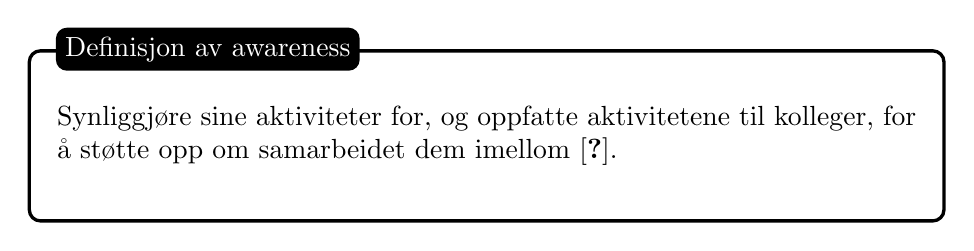
\begin{tikzpicture}
\node [mybox] (box){%
    \begin{minipage}{0.9\textwidth}
     Synliggjøre sine aktiviteter for, og oppfatte aktivitetene til kolleger, for å støtte opp om samarbeidet dem imellom \cite{Randell}.
    \end{minipage}
};
\node[fancytitle, rounded corners, right=10pt] at (box.north west) {Definisjon av awareness};
\end{tikzpicture}%
